%-------------------------------------------------------------------------------
\section{Additional Results}\label{Results}
%-------------------------------------------------------------------------------
This section presents all my results for each of the parameterizations in Table \ref{Parameterizations}. The \textit{exact solution} is constructed using 100,000 random draws for the evaluation of $E\max$ at all states at the true parameter values. The \textit{exact sample} refers to a set of 1,000 simulated agents based on the \textit{exact solution}. As on overall measure of the approximation error, I use the root-mean-square error (RMSE) by comparing the choice probabilities in the \textit{exact sample} to a newly simulated set of 1,000 agents based on the relevant alternative parameterization of the model.
%-------------------------------------------------------------------------------
\subsection{Parameterizations}
%-------------------------------------------------------------------------------
\begin{center}
\begin{threeparttable}
  \caption{Parameterizations}
  \label{Parameterizations}
  \begin{tabular}{crrr}\toprule
  \mc{1}{c}{Parameter} & \mc{1}{r}{Data One} & \mc{1}{r}{Data Two} & \mc{1}{r}{Data Three}  \\
  \midrule
  $\alpha_{10}$         &     9.2100 &     9.2100 &     8.0000 \\
  $\alpha_{11}$         &     0.0380 &     0.4000 &     0.0700 \\
  $\alpha_{12}$         &     0.0330 &     0.0330 &     0.0550 \\
  $\alpha_{13}$         &     0.0005 &     0.0005 &     0.0000 \\
  $\alpha_{14}$         &     0.0000 &     0.0000 &     0.0000 \\
  $\alpha_{15}$         &     0.0000 &     0.0000 &     0.0000 \\
  $\alpha_{20}$         &     8.4800 &     8.2000 &     7.9000 \\
  $\alpha_{21}$         &     0.0700 &     0.0800 &     0.0700 \\
  $\alpha_{22}$         &     0.0670 &     0.0670 &     0.0600 \\
  $\alpha_{23}$         &     0.0010 &     0.0010 &     0.0000 \\
  $\alpha_{24}$         &     0.0220 &     0.0220 &     0.0550 \\
  $\alpha_{25}$         &     0.0005 &     0.0005 &     0.0000 \\
  $\beta_{0}$           &     0.0000 &  5,000.0000 &  5,000.0000 \\
  $\beta_{1}$           &     0.0000 &  5,000.0000 &  5,000.0000 \\
  $\beta_{2}$           &  4,000.0000 & 15,000.0000 & 20,000.0000 \\
  $\gamma_{0}$          & 17,750.0000 & 14,500.0000 & 21,500.0000 \\
  $(\sigma_{11})^{1/2}$ &     0.2000 &     0.4000 &     1.0000 \\
  $\sigma_{12}$         &     0.0000 &     0.0000 &     0.5000 \\
  $\sigma_{13}$         &     0.0000 &     0.0000 &     0.0000 \\
  $\sigma_{14}$         &     0.0000 &     0.0000 &     0.0000 \\
  $(\sigma_{22})^{1/2}$ &     0.2500 &     0.5000 &     1.0000 \\
  $\sigma_{23}$         &     0.0000 &     0.0000 &     0.0000 \\
  $\sigma_{24}$         &     0.0000 &     0.0000 &     0.0000 \\
  $(\sigma_{33})^{1/2}$ &  1,500.0000 &  6,000.0000 &  7,000.0000 \\
  $\sigma_{34}$         &     0.0000 &     0.0000 & $-2.975\times10^7$\\
  $(\sigma_{44})^{1/2}$ &  1,500.0000 &  6,000.0000 &  8,500.0000 \\
  \bottomrule
  \end{tabular}
  %\scriptsize
  %\begin{tablenotes}\item \textbf{Notes:}
  %\end{tablenotes}
\end{threeparttable}
\end{center}\vspace{0.5cm}

%-------------------------------------------------------------------------------
\subsection{Choice Patterns}
%-------------------------------------------------------------------------------
Figure \ref{Choice Patterns} shows the share of agents in the \textit{exact sample} opting for each of the four alternatives by period.\\\newline
\begin{figure}[h!]
\caption{Choice Patterns}\label{Choice Patterns}
\centering
\subfloat[Data One]{
\scalebox{0.30}{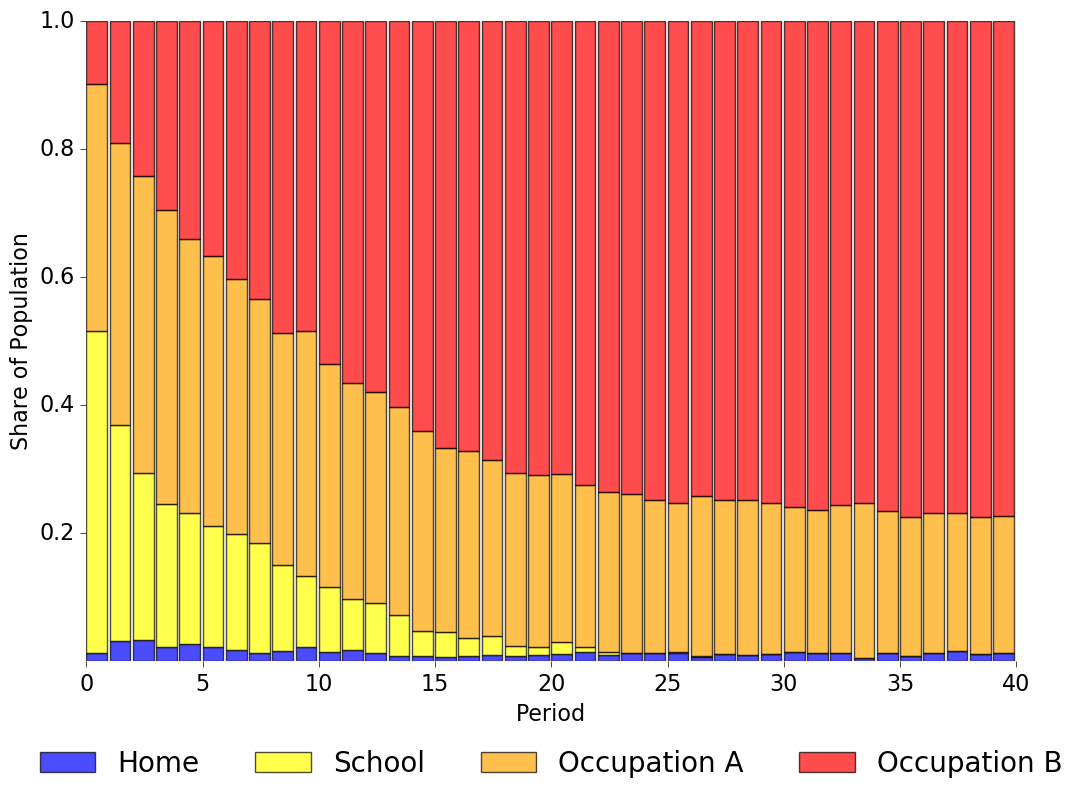
\includegraphics{../material/graph_patterns_one}}}\vspace{0.5cm}
\subfloat[Data Two]{
\scalebox{0.30}{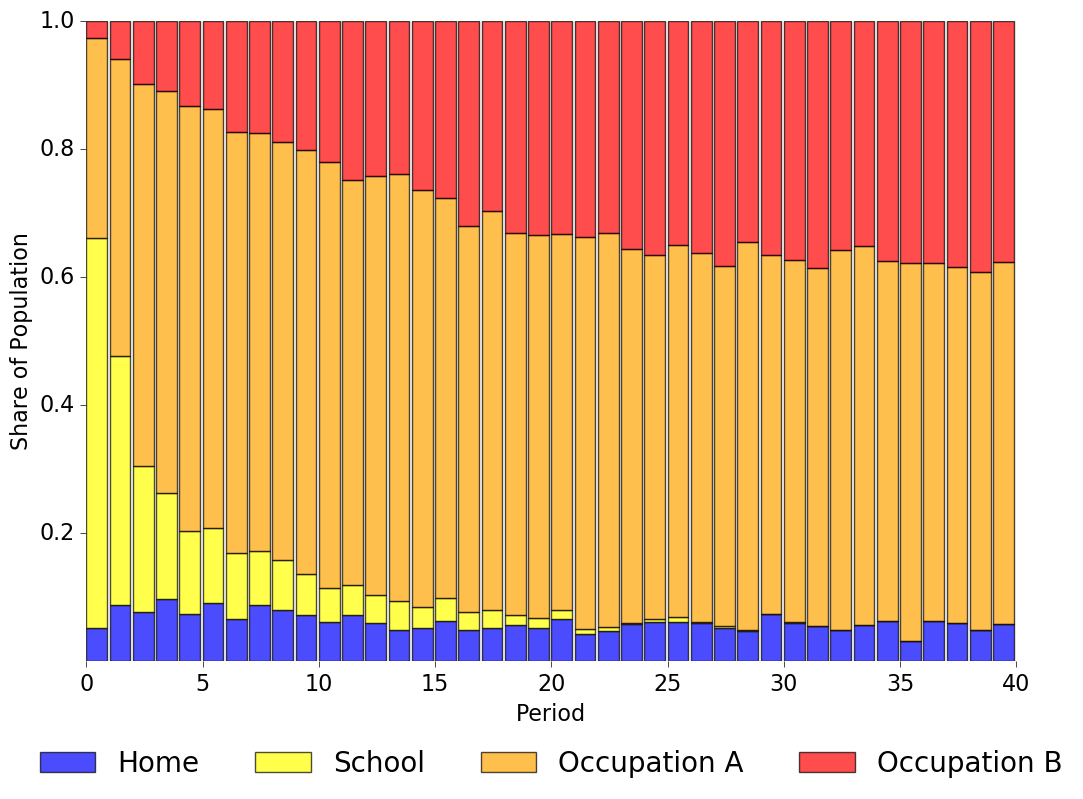
\includegraphics{../material/graph_patterns_two}}}\vspace{0.5cm}
\subfloat[Data Three]{
\scalebox{0.30}{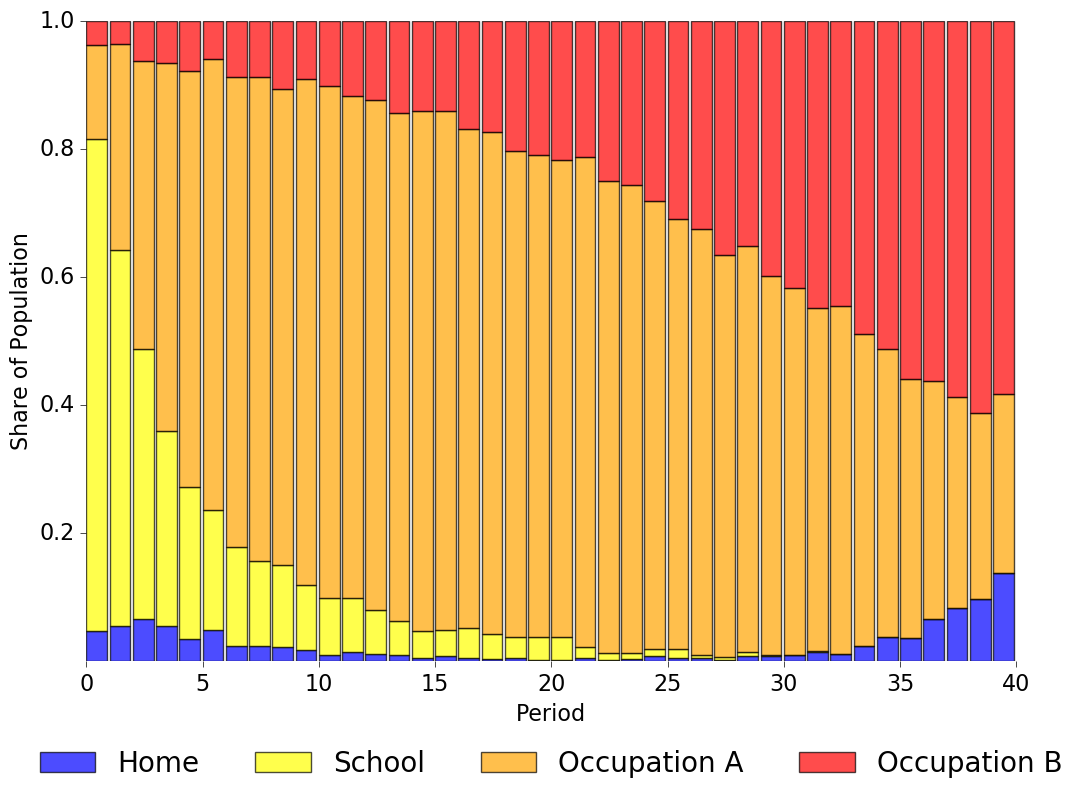
\includegraphics{../material/graph_patterns_three}}} 
\begin{center}
%\begin{minipage}[t]{0.85\columnwidth}\vspace{-0.25cm}
%\item\scriptsize{\textbf{Notes:} }
%\end{minipage}
\end{center}
\end{figure}
\clearpage
%-------------------------------------------------------------------------------
\subsection{Correct Choices}
%-------------------------------------------------------------------------------
Tables \ref{Correct Choices: One} - \ref{Correct Choices: Three} show the proportion of correct choices for alternative interpolation schemes.
\begin{table}[p]\onehalfspacing
\begin{center}
\begin{threeparttable}
  \caption{Correct Choices, Dataset One}
  \label{Correct Choices: One}
  \begin{tabular}{lrrrrr}\toprule
  Points     & All & All & All   & 2,000 & 500   \\
  $E\max$ Draws & 2,000 & 1,000 & 250 & 2,000 & 2,000  \\
  \midrule
  \mc{6}{c}{At Selected Periods} \\
  \midrule
  Period & \mc{5}{c}{} \\
  \phantom{1}1      &  1.000 &  0.998 &  0.938 &  0.967 &  0.942 \\
  10                &  0.990 &  1.000 &  0.989 &  0.988 &  0.979 \\
  20                &  1.000 &  1.000 &  1.000 &  0.998 &  0.999 \\
  30                &  1.000 &  1.000 &  1.000 &  0.994 &  0.998 \\
  40                &  1.000 &  1.000 &  1.000 &  1.000 &  1.000 \\
  Total             &  0.998 &  0.999 &  0.994 &  0.993 &  0.991 \\ % in table 0.9989 and 0.9938
  \midrule
  \mc{6}{c}{Number of Periods over the Lifetime} \\
  \midrule
  Periods & \mc{5}{c}{} \\
  \phantom{0}1 - 10  &   0.000 &  0.000 &  0.000 &  0.000 &  0.000 \\
  11 - 35            &   0.000 &  0.000 &  0.000 &  0.000 &  0.000 \\
  36 - 38            &   0.010 &  0.000 &  0.020 &  0.027 &  0.046 \\
  39                 &   0.036 &  0.043 &  0.181 &  0.190 &  0.252 \\
  40                 &   0.963 &  0.957 &  0.799 &  0.783 &  0.702 \\
  Average            &  39.962 & 39.957 & 39.777 & 39.752 & 39.649 \\
  \bottomrule
  \end{tabular}
\end{threeparttable}
\end{center}
\end{table}

\begin{table}[p]\onehalfspacing
\begin{center}
\begin{threeparttable}
  \caption{Correct Choices, Dataset Two}
  \label{Correct Choices: Two}
  \begin{tabular}{lrrrrr}\toprule
  Points     & All & All & All   & 2,000 & 500   \\
  $E\max$ Draws & 2,000 & 1,000 & 250 & 2,000 & 2,000  \\
  \midrule
  \mc{6}{c}{At Selected Periods} \\
  \midrule
  Period & \mc{5}{c}{} \\
  \phantom{1}1      &  0.998 &  0.994 &  0.993 &  0.996 &  0.988 \\
  10                &  1.000 &  0.998 &  0.995 &  0.990 &  0.972 \\
  20                &  1.000 &  0.997 &  0.994 &  0.979 &  0.961 \\
  30                &  0.998 &  1.000 &  0.998 &  0.988 &  0.989 \\
  40                &  1.000 &  1.000 &  1.000 &  1.000 &  1.000 \\
  Total             &  0.998 &  0.997 &  0.995 &  0.990 &  0.981 \\
  \midrule
  \mc{6}{c}{Number of Periods over the Lifetime} \\
  \midrule
  Periods & \mc{5}{c}{} \\
  \phantom{1}1 - 10 &  0.000 &  0.000 &  0.000 &  0.000 &  0.000 \\
  11 - 35           &  0.000 &  0.000 &  0.000 &  0.001 &  0.001 \\
  36 - 38           &  0.003 &  0.003 &  0.012 &  0.062 &  0.157 \\
  39                &  0.040 &  0.085 &  0.172 &  0.260 &  0.361 \\
  40                &  0.957 &  0.912 &  0.816 &  0.677 &  0.481 \\
  Average           & 39.954 & 39.909 & 39.804 & 39.600 & 39.265 \\
  \bottomrule
  \end{tabular}
\end{threeparttable}
\end{center}
\end{table}

\begin{table}[p]\onehalfspacing
\begin{center}
\begin{threeparttable}
  \caption{Correct Choices, Dataset Three}
  \label{Correct Choices: Three}
  \begin{tabular}{lrrrrr}\toprule
  Points     & All & All & All   & 2,000 & 500   \\
  $E\max$ Draws & 2,000 & 1,000 & 250 & 2,000 & 2,000  \\
  \midrule
  \mc{6}{c}{At Selected Periods} \\
  \midrule
  Period & \mc{5}{c}{} \\
  \phantom{1}1      &  0.995 &  0.993 &  0.985 &  0.991 &  0.979 \\
  10                &  0.995 &  0.995 &  0.982 &  0.975 &  0.931 \\
  20                &  0.995 &  0.997 &  0.994 &  0.979 &  0.940 \\
  30                &  0.994 &  0.999 &  0.989 &  0.974 &  0.972 \\
  40                &  1.000 &  1.000 &  1.000 &  1.000 &  1.000 \\
  Total             &  0.995 &  0.995 &  0.991 &  0.980 &  0.959 \\
  \midrule
  \mc{6}{c}{Number of Periods over the Lifetime} \\
  \midrule
  Periods & \mc{5}{c}{} \\
  \phantom{1}1 - 10 &  0.000 &  0.000 &  0.000 &  0.000 &  0.000 \\
  11 - 35           &  0.000 &  0.000 &  0.000 &  0.003 &  0.030 \\
  36 - 38           &  0.015 &  0.015 &  0.038 &  0.187 &  0.432 \\
  39                &  0.142 &  0.150 &  0.249 &  0.324 &  0.304 \\
  40                &  0.843 &  0.835 &  0.713 &  0.486 &  0.234 \\
  Average           & 39.827 & 39.817 & 39.671 & 39.226 & 38.374 \\
  \bottomrule
  \end{tabular}
\end{threeparttable}
\end{center}\end{table}

%-------------------------------------------------------------------------------
\subsection{Monte Carlo Exercise}
%-------------------------------------------------------------------------------
Tables \ref{Monte Carlo: One} - \ref{Monte Carlo: Three} show the estimation performance for each of the model parameters during the initial Monte Carlo exercise. Let $\theta_i$ denote the true value of parameter $i$, $\hat{\theta}_i$ its average estimate across all Monte Carlo iterations, and $\hat{\theta}_{ij}$ the estimated parameter in iteration $j$. The statistics in the Table \ref{Monte Carlo: One} - \ref{Monte Carlo: Three} are calculated as follows:

\renewcommand\arraystretch{2}
\begin{align*}\begin{array}{l@{\qquad}l}
\text{Bias} & \hat{\theta}_i - \theta_i\\\medskip
\text{$t$ - statistic} & \left(\frac{\hat{\theta}_i - \theta_i}{\sigma_{\hat{\theta_i}}}\right) \sqrt{40} \\
\text{Standard Deviation} & \left[ \frac{1}{39} \sum^{40}_{j = 1} (\hat{\theta}_{ij} - \hat{\theta}_i)^2
\right]^{\tfrac{1}{2}}
\end{array}
\end{align*}
\renewcommand\arraystretch{1}

Note that the table contains the Cholesky decomposition parameters $a_{ij}$ of the covariance matrix of the shocks to the immediate rewards. I report the RMSE, the total number of evaluations of the criterion function, and the number of steps of the optimizer as their average across all 40 Monte Carlo iterations.\\\newline
%
I specify 200 interpolation points, use 500 random draws for the evaluation of $E\max$, and allow for a maximum of 10,000 evaluations of the criterion function by the optimizer for each estimation.\clearpage

\begin{table}\onehalfspacing
\begin{center}
\begin{threeparttable}
  \caption{Monte Carlo Exercise, Dataset One}
  \label{Monte Carlo: One}
  \begin{tabular}{crrrr}\toprule

  Parameter & True Value & Bias & $t$ - statistic & Std. Deviation \\
  \midrule
  $\alpha_{10}$ &     \phantom{20000}9.2100 &    \phantom{-17}0.0012 &     1.6744 &      0.0045 \\
  $\alpha_{11}$ &     0.0380 &      0.0000 &      0.5024 &       0.0006 \\
  $\alpha_{12}$ &     0.0330 &     -0.0002 &     -2.8043 &       0.0003 \\
  $\alpha_{13}$ &     0.0005 &      0.0000 &     12.4900 &       0.0000 \\
  $\alpha_{14}$ &     0.0000 &     -0.0010 &     -4.8287 &       0.0013 \\
  $\alpha_{15}$ &     0.0000 &      0.0000 &      2.1206 &       0.0001 \\
  $\alpha_{20}$ &     8.4800 &     -0.0007 &     -1.2986 &       0.0032 \\
  $\alpha_{21}$ &     0.0700 &     -0.0000 &     -2.1280 &       0.0001 \\
  $\alpha_{22}$ &     0.0670 &     -0.0002 &     -2.3279 &       0.0005 \\
  $\alpha_{23}$ &     0.0010 &      0.0000 &      3.5786 &       0.0000 \\
  $\alpha_{24}$ &     0.0220 &      0.0000 &      2.1136 &       0.0001 \\
  $\alpha_{25}$ &     0.0005 &      0.0000 &      0.5725 &       0.0000 \\
  $\beta_{0}$   &     0.0000 &    -91.0443 &     -4.0973 &     140.5369 \\
  $\beta_{1}$   &     0.0000 &     -7.9753 &     -0.3319 &     151.9692 \\
  $\beta_{2}$   &  4,000.0000 &   -12.2382 &     -0.3042 &     254.4796 \\
  $\gamma_{0}$  & 17,750.0000 &   -60.7969 &     -1.5008 &     256.1998 \\
  $a_{11}$      &     0.2000 &     -0.0009 &     -1.4661 &       0.0040 \\
  $a_{21}$      &     0.0000 &     -0.0011 &     -4.2691 &       0.0016 \\
  $a_{22}$      &     0.2500 &      0.0022 &      3.6085 &       0.0039 \\
  $a_{31}$      &     0.0000 &     -3.6560 &     -0.1081 &     213.8302 \\
  $a_{32}$      &     0.0000 &    -74.1944 &     -3.1560 &     148.6830 \\
  $a_{33}$      &  1,500.0000 &  -219.2507 &     -5.7537 &     241.0047 \\
  $a_{41}$      &     0.0000 &    -41.2545 &     -1.5464 &     168.7276 \\
  $a_{42}$      &     0.0000 &   -174.8974 &     -3.4213 &     323.3108 \\
  $a_{43}$      &     0.0000 &    -32.2724 &     -0.5806 &     351.5762 \\
  $a_{44}$      &  1,500.0000 &  -170.8750 &     -3.5702 &     302.7048 \\
  \midrule
  \mc{1}{l}{Steps}          & 324   & & Evaluations & 1429 \\
  \mc{1}{l}{RMSE}           & 0.0665  & & & \\
  \bottomrule
  \end{tabular}\scriptsize
  \begin{tablenotes}\item \textbf{Notes:} Std. Deviation = Standard Deviation. I calculate the number of steps, number of evaluations, and the RMSE as the average across all 40 Monte Carlo iterations.
  \end{tablenotes}

\end{threeparttable}
\end{center}
\end{table}

\begin{table}\onehalfspacing
\begin{center}
\begin{threeparttable}
  \caption{Monte Carlo Exercise, Dataset Two}
  \label{Monte Carlo: Two}
  \begin{tabular}{crrrr}\toprule

  Parameter & True Value & Bias & $t$ - statistic & Std. Deviation \\
  \midrule
  $\alpha_{10}$ &      \phantom{20000}9.2100 &  -0.0013 & -2.3522 &     0.0036 \\
  $\alpha_{11}$ &      0.0400 &      0.0001 &  1.5572 &    0.0003 \\
  $\alpha_{12}$ &      0.0330 &     -0.0001 & -1.8808 &    0.0003 \\
  $\alpha_{13}$ &      0.0005 &     -0.0000 & -1.2201 &    0.0000 \\
  $\alpha_{14}$ &      0.0000 &     -0.0000 & -0.8527 &    0.0003 \\
  $\alpha_{15}$ &      0.0000 &      0.0000 &  1.2649 &    0.0000 \\
  $\alpha_{20}$ &      8.2000 &     -0.0078 & -5.0148 &    0.0098 \\
  $\alpha_{21}$ &      0.0800 &     -0.0002 & -2.2834 &    0.0005 \\
  $\alpha_{22}$ &      0.0670 &     -0.0001 & -1.9589 &    0.0005 \\
  $\alpha_{23}$ &      0.0010 &      0.0000 & -1.4327 &    0.0000\\
  $\alpha_{24}$ &      0.0220 &      0.0002 &  1.8267 &    0.0006 \\
  $\alpha_{25}$ &      0.0005 &      0.0000 &  4.5655 &    0.0001\\
  $\beta_{0}$   &   5,000.0000 &   -21.6427 & -0.5906 &  231.7552 \\
  $\beta_{1}$   &   5,000.0000 &  -170.0311 & -1.7716 &  607.0113 \\
  $\beta_{2}$   &  15,000.0000 &   218.8722 &  3.3175 &  417.2622 \\
  $\gamma_{0}$  &  14,500.0000 &   -41.7072 & -1.2614 &  209.1211 \\
  $a_{11}$      &      0.4000 &     -0.0401 & -1.4301 &    0.1772 \\
  $a_{21}$      &      0.0000 &      0.0051 &  2.8442 &    0.0114 \\
  $a_{22}$      &      0.5000 &     -0.0028 & -1.9463 &    0.0089 \\
  $a_{31}$      &      0.0000 &    -95.9679 & -2.2467 &  270.1549 \\
  $a_{32}$      &      0.0000 &    106.9453 &  1.5877 &  426.0040 \\
  $a_{33}$      &   6,000.0000 &   132.6752 &  3.3306 &  251.9426 \\
  $a_{41}$      &      0.0000 &     14.5530 &  0.4718 &  195.1054 \\
  $a_{42}$      &      0.0000 &    -82.8807 & -1.7011 &  308.1402 \\
  $a_{43}$      &      0.0000 &   -111.7468 & -2.6635 &  265.3480 \\
  $a_{44}$      &   6,000.0000 &   -38.1595 & -1.4635 &  164.9108 \\
  \midrule
  \mc{1}{l}{Steps}          & 21   & & Evaluations &  460\\
  \mc{1}{l}{RMSE}           & 0.0346  & & & \\
  \bottomrule
  \end{tabular}\scriptsize
  \begin{tablenotes}\item \textbf{Notes:} Std. Deviation = Standard Deviation. I calculate the number of steps, number of evaluations, and the RMSE as the average across all 40 Monte Carlo iterations.
  \end{tablenotes}
\end{threeparttable}
\end{center}
\end{table}

\begin{table}\onehalfspacing
\begin{center}
\begin{threeparttable}
  \caption{Monte Carlo Exercise, Dataset Three}
  \label{Monte Carlo: Three}
  \begin{tabular}{crrrr}\toprule

  Parameter & True Value & Bias & $t$ - statistic & Std. Deviation \\
  \midrule
  $\alpha_{10}$ &    \phantom{20000}8.0000 &   -0.0092 &  -5.3135 &    0.0110 \\
  $\alpha_{11}$ &      0.0700 & -0.0008 & -3.3256 & 0.0016 \\
  $\alpha_{12}$ &      0.0550 & 0.0006 & 1.8263 & 0.0020\\
  $\alpha_{13}$ &      0.0000 & -0.0000 & -0.0452 & 0.0001\\
  $\alpha_{14}$ &      0.0000 & -0.0029 & -5.111  & 0.0036 \\
  $\alpha_{15}$ &      0.0000 & 0.0006 & 5.4264   & 0.0007 \\
  $\alpha_{20}$ &      7.9000 & -0.0039 & -4.3200  & 0.0057    \\
  $\alpha_{21}$ &      0.0700 &  0.0006 & 1.2129  & 0.0031    \\
  $\alpha_{22}$ &      0.0550 & 0.0003 & 1.0699   & 0.0019  \\
  $\alpha_{23}$ &      0.0000 & 0.0000 & 2.4916    & 0.0001 \\
  $\alpha_{24}$ &      0.0600 & -0.0017 & -4.5783    & 0.0023\\
  $\alpha_{25}$ &      0.0000 & -0.0001 & -4.1808  & 0.0001    \\
  $\beta_{0}$   &   5,000.0000 & -40.5552 & -0.3268  & 784.8442  \\
  $\beta_{1}$   &   -5,000.0000 & -25.4629 & -0.2931  & 549.4277  \\
  $\beta_{2}$   &  -20,000.0000 & 9.4701 & 0.0403 & 1487.7457  \\
  $\gamma_{0}$  &   21,500.0000 & 19.3394 & 4.2987 & 28.4534 \\
  $a_{11}$      &      1.0000 & -0.0230 & -3.7447 & 0.0389 \\
  $a_{21}$      &      0.5000 & 0.0040 & 1.2691 & 0.0198  \\
  $a_{22}$      &      0.8660 & -0.0303 & -2.9467  & 0.0651 \\
  $a_{31}$      &      0.0000 & -164.1444 & -1.9570  & 530.4788  \\
  $a_{32}$      &      0.0000 & 722.0474 & 2.3833  & 1916.1160  \\
  $a_{33}$      &   7,000.0000 & 786.9953 & 4.2248  & 1178.1343 \\
  $a_{41}$      &      0.0000 & -88.1003 & -0.5460  & 1020.4223  \\
  $a_{42}$      &      0.0000 & -687.4966 & -2.5796  & 1685.5875  \\
  $a_{43}$      &  -4,250.0000 & -672.5874 & -2.2242  & 1912.5056  \\
  $a_{44}$      &   7,361.2159 & -112.1582 & -0.4167  & 1702.4584  \\
  \midrule
  \mc{1}{l}{Steps}          &  17  & & Evaluations & 421 \\
  \mc{1}{l}{RMSE}           & 0.0249  & & & \\
  \bottomrule
  \end{tabular}\scriptsize
  \begin{tablenotes}\item \textbf{Notes:} Std. Deviation = Standard Deviation. I calculate the number of steps, number of evaluations, and the RMSE as the average across all 40 Monte Carlo iterations.
\end{tablenotes}
\end{threeparttable}
\end{center}
\end{table}
\clearpage
%-------------------------------------------------------------------------------
\subsection{Noise in Criterion Function}\label{Noise in Criterion Function}
%-------------------------------------------------------------------------------
Figure \ref{Criterion Functions} shows the exact and approximate criterion function around the true parameter values. To get a sense of a possible discrepancy between the two, I perturb $\beta_1$ around its true value in \$100 increments. This parameter captures the effect of tuition cost on educational enrollment and is of particular interest for the ex ante evaluation of tuition policies.\footnote{See \citet{Keane.1997} and \citet{Keane.2001} for examples.} While the exact criterion function has its minimum at the actual value, this is not true for the approximated function. The latter attains its minimum at a perturbation of -\$100. This casts doubt on the quality of the approximation. \begin{figure}[h!]
\caption{Criterion Functions}\label{Criterion Functions}
\centering
\scalebox{0.30}{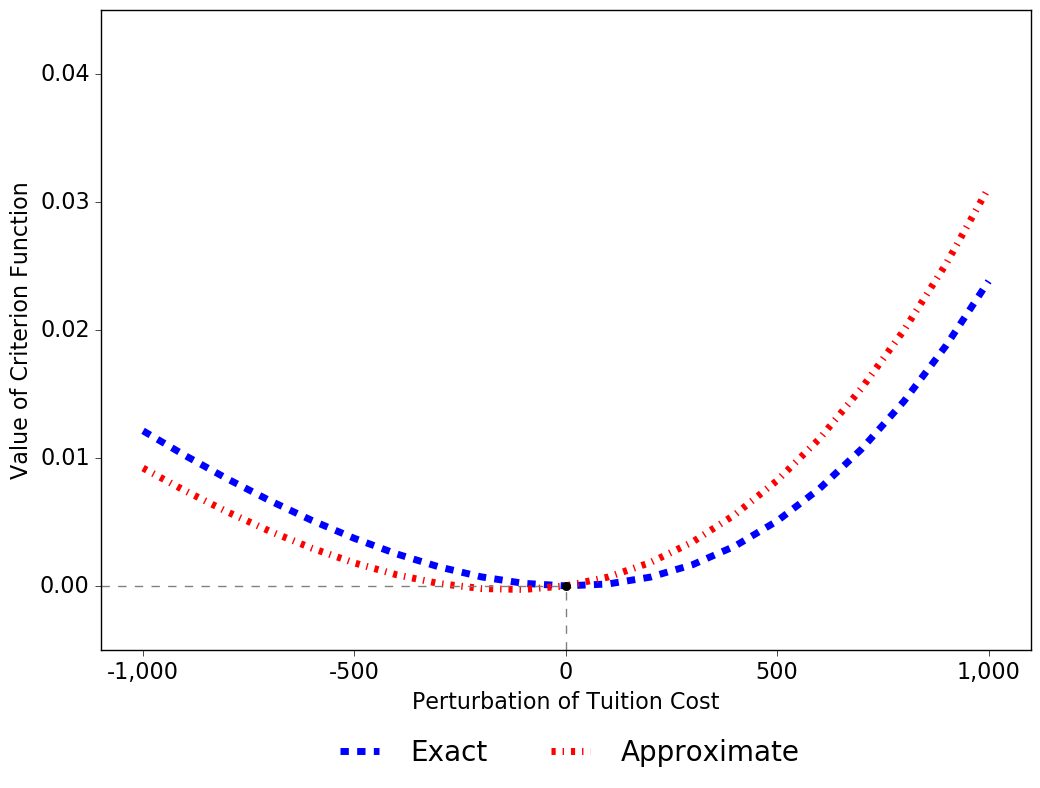
\includegraphics{../material/graph_criterions.png}}\vspace{0.5cm}
\end{figure}

%-------------------------------------------------------------------------------
\subsection{Interpolation Schemes}\label{Appendix Interpolation Schemes}
%-------------------------------------------------------------------------------
Table \ref{Interpolation Schemes} repeats the estimation results based on alternative interpolation schemes. I use a single processor to ensure comparability of computation times. Table \ref{Static Estimation} shows the estimated parameter values from the misspecified static estimation that provides the starting values for the Monte Carlo Exercise. I solve the DP problem at all states and use 500 random draws for the evaluation of $E\max$. I allow for a maximum of 1,000 evaluations of the criterion function by the optimizer which terminates after 284 steps. Each Monte Carlo iteration starts with a RMSE of 0.16.\begin{table}\onehalfspacing
\begin{center}
\begin{threeparttable}
  \captionsetup{width=30cm}
  \caption{Interpolation Schemes}
  \label{Interpolation Schemes}
  \begin{tabular}{lrrrr}\toprule
  Points      & 200 & 500 & 1,500  & All \\
  $E\max$ Draws & 500 &  500 &   500 & 500 \\
  \midrule
  RMSE        & 0.10 &   0.09 &    0.07 &  0.03  \\
  Minutes     &  35 &      96 &    361 &   794 \\
  Steps       &  1,090 &   2,671 &   5,730 &  32,774 \\
  Evaluations & 3,017 &   6,412 &    12,020 & 59,680 \\ %why steps and evals switched in old?
  \bottomrule
  \end{tabular}\scriptsize
  \begin{tablenotes}\item \textbf{Notes:} All results are calculated as the average across all 40 Monte Carlo iterations.
  \end{tablenotes}
  \end{threeparttable}
  \end{center}
\end{table}
\begin{table}\onehalfspacing
\begin{center}
\begin{threeparttable}
  \caption{Static Estimation}
  \label{Static Estimation}
  \begin{tabular}{crr}\toprule
  \mc{1}{c}{Parameter} & \mc{1}{r}{True} & \mc{1}{r}{Estimated}  \\
  \midrule
  $\alpha_{10}$         &     9.2100 &     9.1731      \\
  $\alpha_{11}$         &     0.0380 &     0.0369        \\
  $\alpha_{12}$         &     0.0330 &     0.0353       \\
  $\alpha_{13}$         &     0.0005 &     0.0005       \\
  $\alpha_{14}$         &     0.0000 &     0.0006  \\
  $\alpha_{15}$         &     0.0000 &     0.0001  \\
  $\alpha_{20}$         &     8.4800 &     8.7721  \\
  $\alpha_{21}$         &     0.0700 &     0.0698  \\
  $\alpha_{22}$         &     0.0670 &     0.0524  \\
  $\alpha_{23}$         &     0.0010 &     0.0010   \\
  $\alpha_{24}$         &     0.0220 &     0.0265  \\
  $\alpha_{25}$         &     0.0005 &     0.0011  \\
  $\beta_{0}$           &     0.0000 &   -73.7137   \\
  $\beta_{1}$           &     0.0000 &  -132.6122   \\
  $\beta_{2}$           &  4,000.0000 & -6,586.5820   \\
  $\gamma_{0}$          & 17,750.0000 & 17,703.5550   \\
  $a_{11}$              &     0.2000 &     0.2292   \\
  $a_{21}$              &     0.0000 &     0.0030   \\
  $a_{22}$              &     0.2500 &     0.2472  \\
  $a_{31}$              &     0.0000 &     -12,619.6009 \\
  $a_{32}$              &     0.0000 &     320.4472  \\
  $a_{33}$              & 1,500.0000 &     1,590.5971  \\
  $a_{41}$              &     0.0000 &     33.5865  \\
  $a_{42}$              &     0.0000 &  3,048.3204   \\
  $a_{43}$              &     0.0000 &     -39.6065\\
  $a_{44}$              &  1,500.0000 &   1505.0728 \\
  \midrule
  \mc{1}{l}{Steps}          & \mc{2}{c}{284} \\
  \mc{1}{l}{Evaluations}    & \mc{2}{c}{1,000}\\
  \bottomrule
 \end{tabular}
  %\scriptsize
  %\begin{tablenotes}\item \textbf{Notes:}
  %\end{tablenotes}
\end{threeparttable}
\end{center}
\end{table}

